
\setcounter{chapter}{1}
\chapter{Business understanding and project requirements}
\label{ch:business_understanding}
\minitoc %insert la minitoc
\graphicspath{{Chapitre2/figures/}}

%\DoPToC

%==============================================================================
\pagestyle{fancy}
\fancyhf{}
\fancyhead[R]{\bfseries\rightmark}
\fancyfoot[R]{\thepage}
\renewcommand{\headrulewidth}{0.5pt}
\renewcommand{\footrulewidth}{0pt}
\renewcommand{\chaptermark}[1]{\markboth{\MakeUppercase{\chaptername~\thechapter. #1 }}{}}
\renewcommand{\sectionmark}[1]{\markright{\thechapter.\thesection~ #1}}

\begin{spacing}{1.2}
%==============================================================================

\section*{Introduction}
This chapter establishes the theoretical and contextual foundation of the project. It begins with an overview of AI technologies such as Large Language Models (LLMs), Generative AI, and AI agents, highlighting their relevance to modern software engineering. Next, it presents the state of the art by reviewing existing solutions for code quality and best practices. Finally, it defines the project requirements, showing how this work addresses gaps by integrating AI-driven assistance into key development phases.

\section{Foundations and Motivation}

\subsection{Foundational AI Concepts}
Artificial Intelligence (AI) refers to computational systems capable of performing tasks that typically require human intelligence, including reasoning, learning, problem-solving, and decision-making~\cite{ai2024definition}. AI encompasses a wide range of techniques with distinct capabilities and applications. Figure~\ref{fig:ai_hierarchy} illustrates a hierarchy of AI technologies.

\begin{figure}[H]
\centering
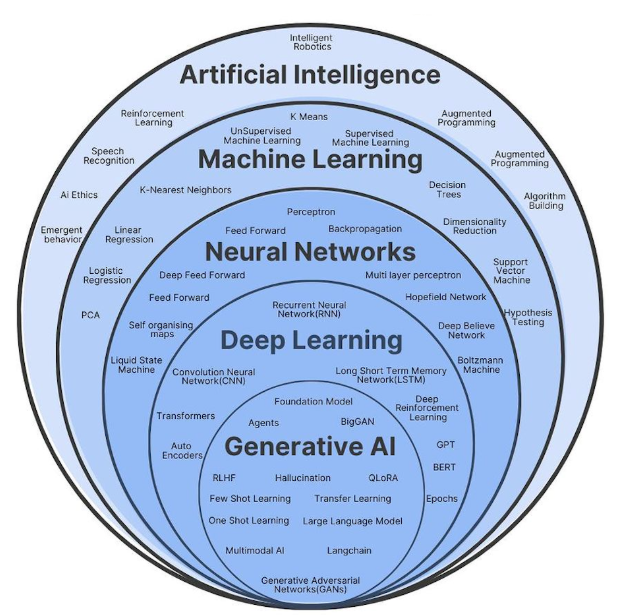
\includegraphics[scale=0.6]{Images/AI.png}
\caption{Hierarchy of AI Technologies}
\label{fig:ai_hierarchy}
\end{figure}

Key categories include:

\begin{itemize}
\item \textbf{Symbolic AI:} Rule-based reasoning and knowledge representation systems.
\item \textbf{Machine Learning (ML):} Algorithms that learn from data to improve task performance~\cite{ml2024definition}.
\item \textbf{Deep Learning (DL):} Neural networks with multiple layers capable of modeling complex patterns~\cite{dl2024definition}.
\item \textbf{Generative AI:} Systems that produce new content, such as text or code, by learning patterns from existing datasets~\cite{generative_ai2024}.
\end{itemize}

\subsubsection{Large Language Models (LLMs)}
LLMs represent a breakthrough in generative AI, trained on extensive natural language and code corpora~\cite{llm2024breakthrough}. Unlike traditional tools, LLMs understand context, semantics, and intent, enabling complex reasoning across domains. Figure~\ref{fig:llm_overview} provides a chronological overview of LLM development from 2018–2024.

\begin{figure}[H]
\centering
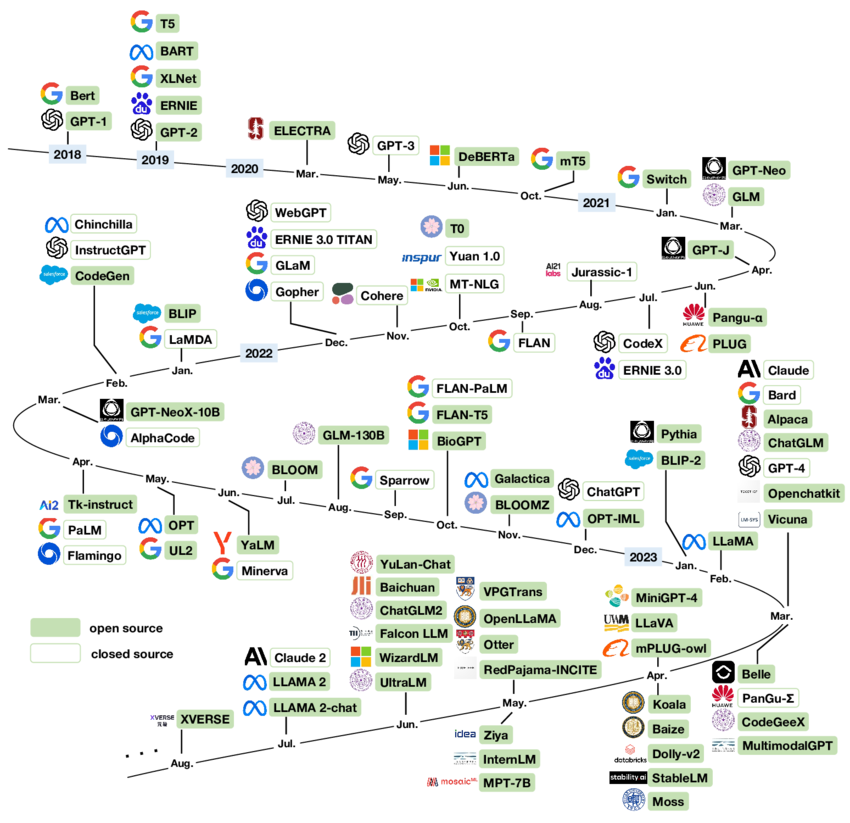
\includegraphics[scale=1]{Images/A-chronological-overview-of-large-language-models-LLMs-multimodal-and-scientific.png}
\caption{Chronological Overview of Large Language Models (LLMs)}
\label{fig:llm_overview}
\end{figure}

LLM capabilities include:

\begin{itemize}
\item \textbf{Natural Language Understanding}
\item \textbf{Pattern Recognition}
\item \textbf{Content Generation}
\item \textbf{Reasoning and Inference}
\end{itemize}

In software development, these capabilities translate into:

\begin{itemize}
\item \textbf{Contextual Code Analysis}
\item \textbf{Intelligent Code Generation}
\item \textbf{Explanatory Documentation}
\item \textbf{Semantic Standards Enforcement}
\end{itemize}

\subsubsection{AI Agents}
AI agents build on LLMs by autonomously reasoning, planning, and executing development tasks. They orchestrate LLM capabilities within workflows, providing seamless integration into IDEs, testing frameworks, and version control systems. Figure~\ref{fig:ai_agent_workflow} illustrates a typical AI agent architecture and orchestration workflow.

\begin{figure}[H]
\centering
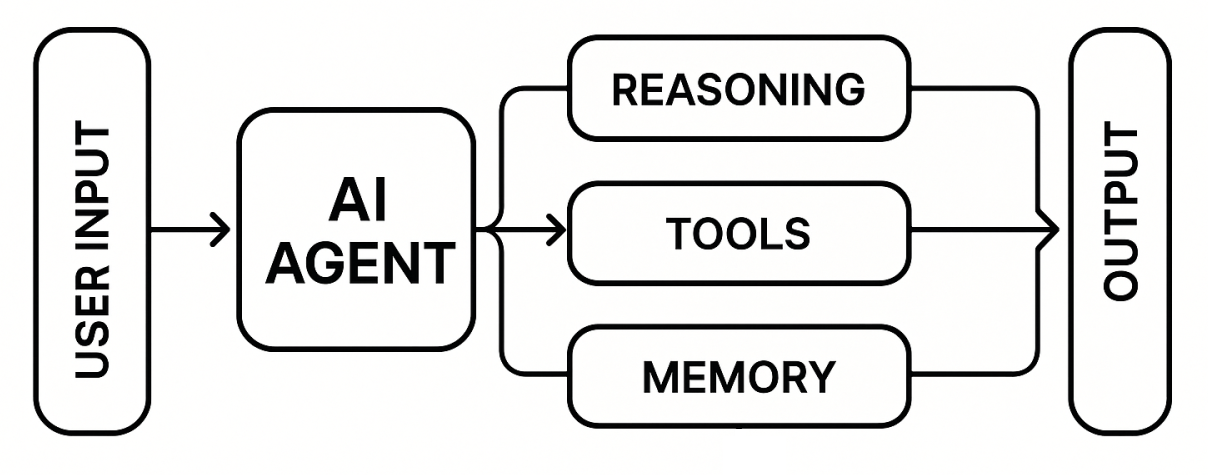
\includegraphics[scale=0.2]{Images/ai_agent.png}
\caption{AI Agent Architecture and Orchestration Workflow}
\label{fig:ai_agent_workflow}
\end{figure}

Core components include:

\begin{itemize}
\item Code Analysis Engine
\item Contextual Reasoning
\item Development Tool Integration
\item Contextual Adaptation via system prompts
\item Feedback and Explanation System
\end{itemize}

\paragraph{Balancing AI Capabilities and Practical Considerations}
While LLM-powered systems provide strong \textit{capabilities}—contextual understanding, automated analysis, and project-specific adaptation—they also present \textit{practical constraints}, including computational cost, context window limits, accuracy variability, and integration complexity. The system design explicitly navigates these trade-offs to deliver reliable, low-latency guidance directly inside the IDE.

\subsection{The AI Revolution in Software Engineering}
Modern software development faces increasing complexity. Traditional practices often struggle to maintain code quality while meeting deadlines. AI technologies offer transformative opportunities by embedding intelligent assistance directly into the development workflow.

Industry adoption highlights this impact: surveys show AI-generated code accounts for a growing portion of development output in major organizations~\cite{google2024ai_code, google2024developer_survey}. AI integration addresses critical challenges such as maintaining code quality, reducing technical debt, and scaling development practices across teams.

\subsubsection{AI-Enhanced SDLC}
The AI-enhanced Software Development Life Cycle (SDLC) embeds intelligent assistance throughout all phases, directly influencing planning, design, coding, testing, and deployment.

Its transformative impact on development practices includes:

\begin{itemize}
\item \textbf{From Reactive to Proactive:} Feedback is delivered continuously during coding and design, preventing issues before they require refactoring.
\item \textbf{From Inconsistent to Scalable:} AI agents provide uniform, expert-level guidance across teams and codebases.
\item \textbf{From Static to Adaptive:} AI adapts to project-specific patterns, team preferences, and evolving best practices.
\item \textbf{From Isolated to Integrated:} Guidance is embedded within workflows rather than treated as a separate phase, bridging planning, implementation, testing, and maintenance.
\end{itemize}

\subsubsection{AI Applications Across the SDLC}
AI can support specific phases of the SDLC as follows:

\begin{itemize}
\item \textbf{Requirements and Planning:} Estimate timelines, identify ambiguities, and translate requirements into technical specifications.
\item \textbf{Design and Architecture:} Recommend patterns, detect anti-patterns, and ensure compliance with organizational standards.
\item \textbf{Implementation:} Context-aware code completion, best practice enforcement, bug detection, and refactoring guidance.
\item \textbf{Testing and Quality Assurance:} Generate test cases, identify edge cases, and prioritize test execution.
\item \textbf{Deployment and Maintenance:} Monitor performance, predict issues, and recommend optimizations.
\end{itemize}

Overall, the AI-enhanced SDLC shifts development from reactive, fragmented practices to a proactive, adaptive, and integrated approach. This aligns directly with the goals of this project: delivering real-time, framework-specific guidance within the IDE to improve developer efficiency and maintain code quality.

\section{State of the Art and Existing Solutions}

Building on the foundations above, this section examines both market-available solutions and environment-specific approaches to understand the current landscape of code quality enforcement and developer assistance, identifying gaps that the proposed solution aims to fill.

\subsection{State of the Art}

The software development market offers a variety of AI-powered tools and platforms designed to enhance code quality and developer productivity. These solutions represent the current state of the art in intelligent development assistance.

\subsubsection{AI-Powered Code Analysis Tools}
Key categories include:

\begin{itemize}
\item \textbf{AI Code Assistants:} GitHub Copilot, Amazon CodeWhisperer, and Tabnine provide AI-powered code completion and generation, helping developers write code more efficiently.
\item \textbf{AI-Powered IDEs:} Tools like Cursor and Claude Code integrate AI assistance directly into the coding workflow, offering context-aware code generation, refactoring, and intelligent suggestions.
\item \textbf{Static Analysis Platforms:} Solutions such as SonarQube, CodeClimate, and DeepCode offer automated code quality analysis with AI-enhanced pattern detection.
\item \textbf{AI Code Review Tools:} Platforms like PullRequest.com and CodeRabbit provide AI-assisted code review, offering automated suggestions and quality assessments.
\end{itemize}

\subsubsection{Capabilities of Market Solutions}
Typical features include:

\begin{itemize}
\item \textbf{General Code Analysis:} Broad pattern recognition and quality assessment across multiple languages and frameworks.
\item \textbf{AI-Powered Suggestions:} Recommendations for code improvements, refactoring, and general best practices.
\item \textbf{IDE Integration:} Seamless integration with widely used environments such as VS Code, IntelliJ, and Eclipse.
\end{itemize}

\subsection{Existing Environment-Specific Approaches}

Within our development environment, software engineers rely on a combination of modern AI-powered tools and traditional mechanisms to maintain code quality.

\subsubsection{Current Feedback Mechanisms}

\begin{itemize}
\item \textbf{Code Reviews:} Human reviewers provide context-aware feedback on design quality, readability, maintainability, and adherence to standards. Feedback is high-level but often delayed and resource-intensive.
\item \textbf{Presubmit Checks:} Automated scripts enforce style guides, compilation correctness, and basic safety constraints. They are fast but primarily focus on surface-level checks.
\item \textbf{Coding Assistant:} Internal IDE features AI-powered code completion, generation, and basic suggestions.
\item \textbf{Linters:} IDE-integrated linters provide real-time style and deprecation warnings but do not enforce complex best practices.
\item \textbf{Rule-Based Checks:} Enforce coding conventions and naming schemes consistently but cannot reason about complex or context-dependent practices.
\end{itemize}

\subsubsection{Gap Analysis: Market vs. Environment Solutions}

While both market solutions and environment-specific approaches provide valuable capabilities, they leave significant gaps in enforcing internal framework-specific best practices during the coding phase.

\paragraph{Limitations of Market Solutions}

\begin{itemize}
\item \textbf{Generic Analysis:} Lack deep understanding of internal framework-specific conventions.
\item \textbf{External Dependency:} May require sharing internal code, posing security or privacy concerns.
\item \textbf{Limited Customization:} Cannot easily enforce project-specific practices or architectural patterns.
\end{itemize}

\paragraph{Limitations of Environment Solutions}

\begin{itemize}
\item Coding Assistant and linters focus on general guidance, not framework-specific practices.
\item Rule-based and presubmit checks are reactive rather than proactive, offering feedback after coding rather than during authoring.
\end{itemize}

Figure~\ref{fig:developer_workflow_feedback_timeline} illustrates how current mechanisms provide feedback at different points in the workflow, highlighting the gap during active coding.

\begin{figure}[H]
\centering
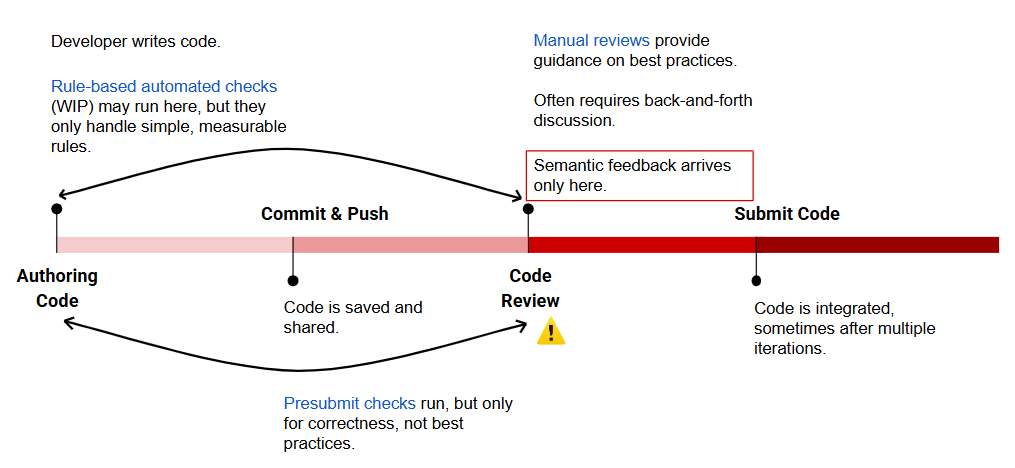
\includegraphics[scale=0.9]{Images/developer_workflow_feedback_timeline.png}
\caption{Current Developer Workflow Feedback Timeline}
\label{fig:developer_workflow_feedback_timeline}
\end{figure}

\subsubsection{Impact of Delayed Feedback}

The current workflow introduces several challenges:

\begin{itemize}
\item \textbf{Technical Debt Accumulation:} Delayed feedback leads to inconsistencies and long-term maintenance costs.
\item \textbf{Prolonged Review Cycles:} Multiple iterations are required to fix issues discovered late.
\item \textbf{Developer Frustration:} Repetitive corrections decrease productivity.
\item \textbf{Inconsistent Quality Standards:} Lack of real-time guidance leads to variable adherence across teams.
\item \textbf{Increased Costs:} Late discovery of issues exponentially increases remediation effort.
\end{itemize}

\subsection{Opportunity for Framework-Specific AI Solutions}

The analysis reveals a clear opportunity for integrating framework-specific AI solutions. Combining the intelligence of market tools with the specificity required for internal frameworks, these solutions can deliver real-time, context-aware guidance directly in the coding phase.

Such a solution addresses the observed gap:

\begin{itemize}
\item Real-time adherence to internal framework best practices.
\item Integration directly into the developer workflow.
\item Proactive feedback that reduces review effort and technical debt.
\end{itemize}

This motivates the development of an LLM-powered, IDE-integrated assistant that provides intelligent, framework-aware support, complementing existing tools while filling the critical gap in real-time guidance.
\section{Project Requirements}

We now translate the identified opportunity into concrete requirements. The proposed solution integrates LLM-powered assistance directly into the developer workflow within the IDE to provide real-time, actionable guidance while maintaining performance, usability, and scalability.

\subsection{Motivation for Use Case Analysis}

Understanding how developers will interact with the system is critical for designing effective functionality. Use case analysis provides a structured approach to capture user-system interactions, identify key actors, and define the boundaries of the system. This ensures that the system delivers targeted support precisely where it is needed during the active coding phase.

\subsubsection{System Use Cases}
\begin{figure}[H]
    \centering
    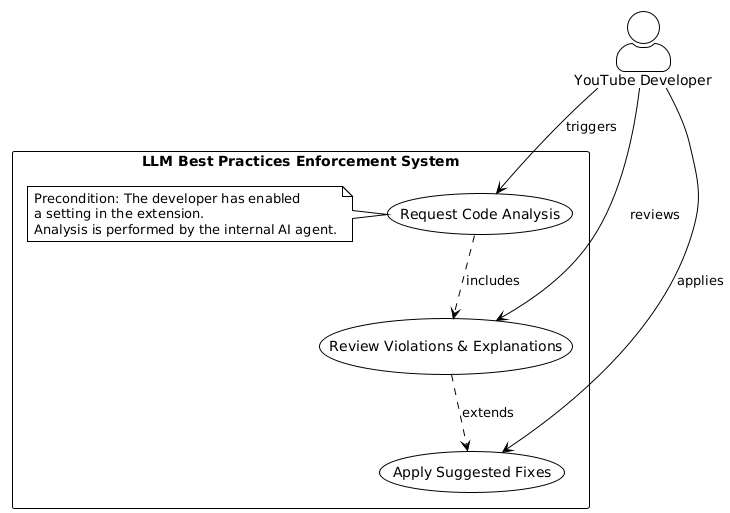
\includegraphics[scale=0.5]{images/use_case_diagram.png}
    \caption{System Use Case Diagram}
    \label{fig:use_case_diagram}
    \end{figure}

Figure~\ref{fig:use_case_diagram} illustrates the core functionality of the system from the perspective of YouTube developers. The primary actor is the \textbf{YouTube Developer}, who interacts with the system through three main use cases:

\begin{enumerate}
\item \textbf{Request Code Analysis:} Trigger real-time evaluation of code for adherence to framework best practices.
\item \textbf{Review Violations and Explanations:} Inspect flagged violations, with clear, context-specific explanations provided by the system.
\item \textbf{Apply Suggested Fixes (Optional):} Accept, modify, or reject actionable AI-generated suggestions to improve code quality.
\end{enumerate}

This design ensures that developers remain in control of their workflow while benefiting from comprehensive, intelligent feedback. Optional scenarios, such as applying fixes, allow flexibility and respect developer autonomy. The use case diagram focuses on core interactions, leaving authentication and administrative workflows out of scope.

\subsection{Functional Requirements}

Based on the use cases and the gaps identified in existing tools, the system must provide the following core functionalities:

\begin{itemize}
\item \textbf{Detect Framework Violations:} Identify violations of internal YouTube framework best practices in real-time.
\item \textbf{Provide Contextual Explanations:} Deliver developer-friendly explanations that clarify why a particular pattern is problematic.
\item \textbf{Generate Actionable Fixes:} Suggest concrete AI-driven solutions aligned with framework conventions.
\item \textbf{Enable Developer Interaction:} Allow developers to accept, reject, or modify suggested fixes, maintaining workflow control.
\item \textbf{Maintain Contextual Relevance:} Ensure feedback remains accurate and properly anchored as code evolves.
\item \textbf{Seamless IDE Integration:} Embed within the existing internal IDE without disrupting normal development processes.
\end{itemize}

\subsection{Non-Functional Requirements}

In addition to core functionality, the system must satisfy broader quality criteria:

\begin{itemize}
\item \textbf{Performance:} Provide near real-time feedback to avoid interrupting workflow.
\item \textbf{Scalability:} Efficiently handle large codebases and multiple simultaneous users.
\item \textbf{Maintainability:} Support modular updates, addition of new rules, and AI model improvements.
\item \textbf{Reliability:} Operate robustly in production with minimal downtime.
\item \textbf{Security and Privacy:} Comply with organizational policies, safeguarding code and data.
\item \textbf{Usability:} Deliver concise, context-aware, and minimally intrusive feedback.
\item \textbf{Extensibility:} Allow easy addition of new rules, models, or integrations.
\end{itemize}

Table~\ref{tab:extended_requirements} summarizes functional and non-functional requirements.

\begin{table}[H]
\centering
\caption{Summary of Project Requirements}
\label{tab:extended_requirements}
\begin{tabular}{|p{3cm}|p{11cm}|}
\hline
\textbf{Requirement Type} & \textbf{Description} \\
\hline
Functional & Detection, explanations, fixes, interaction, context, IDE integration \\
\hline
Non-Functional & Performance, scalability, maintainability, reliability, security, usability, extensibility \\
\hline
\end{tabular}
\end{table}


These requirements directly address the gaps identified in both market and environment-specific solutions. By embedding proactive, context-aware feedback into the coding workflow, the system:

\begin{itemize}
\item Reduces framework-specific errors during development.
\item Improves adherence to YouTube internal standards.
\item Enhances developer productivity by providing guidance in real-time.
\end{itemize}

The use case analysis connects these requirements to real developer interactions, ensuring that the system’s functionality aligns with actual workflow needs and supports effective adoption.

\section*{Conclusion}

This chapter formalizes the project requirements, bridging the gap between the problem analysis and system design. It introduces the rationale for capturing developer interactions via use cases, defines functional and non-functional requirements, and establishes concrete acceptance criteria. Together, these elements provide a solid foundation for the subsequent system design chapter.






%==============================================================================
\end{spacing}


